\documentclass{article}
\usepackage{amsmath}
\usepackage{amssymb}
\usepackage{graphicx}

\setcounter{MaxMatrixCols}{11}

\graphicspath{ {./images/} }

\title{Camera Model and Calibration}
\author{David Robinson}
\date{}
\setlength{\parindent}{0pt}

\begin{document}
\maketitle

\section*{Applications}
\subsection*{Object Transfer}
Transfer an object from one image or video to another. For example, inserting a person and their
shadow from one video to another.

\subsection*{Pose Estimation}
Given a 3D model of an object and its image (2D projection), determine the location and orientation
(translation and rotation) of the object, such that when projected on the image plane, it will
match the image.

\section*{Perspective Projection}
\subsubsection*{Origin at the lens center}
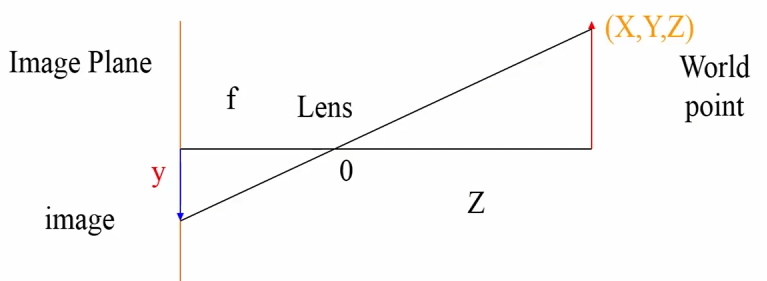
\includegraphics[scale=0.65]{perspective_lens.png}

\[\frac{-y}{Y}=\frac{f}{Z}\rightarrow y=-\frac{fY}{Z}\quad\quad \frac{-x}{X}=\frac{f}{Z}\rightarrow
x =-\frac{fX}{Z}\]

\subsubsection*{Origin at the image center}
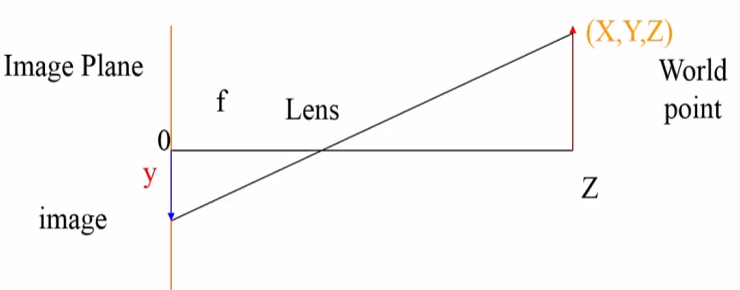
\includegraphics[scale=0.5]{perspective_image.png}

\[\frac{-y}{Y}=\frac{f}{Z-f}\rightarrow y=-\frac{fY}{Z-f}\quad\quad \frac{-x}{X}=
\frac{f}{Z-f}\rightarrow x =-\frac{fX}{Z-f}\]

\section*{Transformations}
\subsection*{3D Translation}
\[\begin{bmatrix}
    X_2 \\ Y_2 \\ Z_2
\end{bmatrix} = \begin{bmatrix}
    X_1 \\ Y_1 \\ Z_1
\end{bmatrix} + \begin{bmatrix}
    d_x \\ d_y \\ d_z
\end{bmatrix}\]

\[\begin{bmatrix}
    X_2 \\ Y_2 \\ Z_2 \\ 1
\end{bmatrix} = T \begin{bmatrix}
    X_1 \\ Y_1 \\ Z_1 \\ 1
\end{bmatrix}\] where $T=\begin{bmatrix}
    1 & 0 & 0 & d_x \\
    0 & 1 & 0 & d_y \\
    0 & 0 & 1 & d_z \\
    0 & 0 & 0 & 1
\end{bmatrix}$ is the translation matrix

\pagebreak

\subsection*{Scaling}
\[\begin{bmatrix}
    X_2 \\ Y_2 \\ Z_2
\end{bmatrix} = \begin{bmatrix}
    X_1 \times S_x \\ Y_1 \times S_y \\ Z_1 \times S_z
\end{bmatrix}\]

\[\begin{bmatrix}
    X_2 \\ Y_2 \\ Z_2 \\ 1
\end{bmatrix} = S \begin{bmatrix}
    X_1 \\ Y_1 \\ Z_1 \\ 1
\end{bmatrix}\] where $S=\begin{bmatrix}
    S_x & 0 & 0 & 0 \\
    0 & S_y & 0 & 0 \\
    0 & 0 & S_z & 0 \\
    0 & 0 & 0 & 1
\end{bmatrix}$ is the scaling matrix

\subsection*{Rotation}
Rotation matrices are orthonormal matrices, so the inverse and transpose of a rotation matrix are
equal.
\[r_i \cdot r_j = \begin{cases}
    1 & \text{if } i = j \\
    0 & \text{otherwise}
\end{cases}\] where $r_i$ and $r_j$ are rows in the rotation matrix.

\vspace{1em}

\subsubsection*{Rotation around $Z$ axis:}
\[\begin{bmatrix}
    X_2 \\ Y_2 \\ Z_2
\end{bmatrix} = R \begin{bmatrix}
    X_1 \\ Y_1 \\ Z_1
\end{bmatrix}\] where $R=\begin{bmatrix}
    \cos\theta & -\sin\theta & 0 \\
    \sin\theta & \cos\theta & 0 \\
    0 & 0 & 1
\end{bmatrix}$ is the rotation matrix

\subsubsection*{Rotation around an arbitrary axis:}
\[R=R_Z^\alpha R_Y^\beta R_Z^\gamma=\begin{bmatrix}
    \cos\alpha\cos\beta & \cos\alpha\sin\beta\sin\gamma - \sin\alpha\cos\gamma &
    \cos\alpha\sin\beta\cos\gamma + \sin\alpha\sin\gamma \\
    \sin\alpha\cos\beta & \sin\alpha\sin\beta\sin\gamma + \cos\alpha\cos\gamma &
    \sin\alpha\sin\beta\cos\gamma - \cos\alpha\sin\gamma \\
    -\sin\beta & \cos\beta\sin\gamma & \cos\beta\cos\gamma
\end{bmatrix}\]

The approximation if angles are small ($\cos\theta \approx 1$) is:
\[\begin{bmatrix}
    1 & -\alpha & \beta \\
    \alpha & 1 & -\gamma \\
    -\beta & \gamma & 1
\end{bmatrix}\]

\subsection*{Perspective}
\textbf{Homogenous transformation}
\[(X, Y, Z) \rightarrow (kX, kY, kZ, k)\]
\textbf{Inverse Homogenous transformation}
\[(C_{h1}, C_{h2}, C_{h3}, C_{h4}) \rightarrow \Big(\frac{C_{h1}}{C_{h4}}, \frac{C_{h2}}{C_{h4}},
\frac{C_{h3}}{C_{h4}}\Big)\]

\[\begin{bmatrix}
    C_{h1} \\ C_{h2} \\ C_{h3} \\ C_{h4}
\end{bmatrix} = P \begin{bmatrix}
    kX \\ kY \\ kZ \\ k
\end{bmatrix}=\begin{bmatrix}
    kX \\ kY \\ kZ \\ k - \frac{kZ}{f}
\end{bmatrix}\] where $P=\begin{bmatrix}
    1 & 0 & 0 & 0 \\
    0 & 1 & 0 & 0 \\
    0 & 0 & 1 & 0 \\
    0 & 0 & \frac{-1}{f} & 1
\end{bmatrix}$ is the perspective matrix

\[x=\frac{C_{h1}}{C_{h4}}=\frac{kX}{k-\frac{kZ}{f}}=\frac{fX}{f-Z}\]
\[y=\frac{C_{h2}}{C_{h4}}=\frac{kY}{k-\frac{kZ}{f}}=\frac{fY}{f-Z}\]

\section*{Camera Model}
\begin{enumerate}
    \item Camera is at the origin of the world coordinates
    \item Translate by $G$
    \item Rotate around $Z$ axis in counter clockwise direction
    \item Rotate again around $X$ in counter clockwise direction
    \item Translate by $C$
\end{enumerate}
Since we are moving the camera instead of object we need to use inverse transformations.
\[C_h=P T_C R_{-\phi}^X R_{-\theta}^Z T_G W_h\]

Using the previous values for $P$, $C$, and $R$:
\[x=f\frac{(X-X_0)\cos\theta + (Y-Y_0)\sin\theta - r_1}{-(X-X_0)\sin\theta\sin\phi +
(Y-Y_0)\cos\theta\sin\phi - (Z-Z_0)\cos\phi + r_3 + f}\]
\[y=f\frac{(X-X_0)\sin\theta\cos\phi + (Y-Y_0)\cos\theta\cos\phi + (Z-Z_0)\sin\phi -
r_2}{-(X-X_0)\sin\theta\sin\phi + (Y-Y_0)\cos\theta\sin\phi - (Z-Z_0)\cos\phi + r_3 + f}\]

\subsection*{Camera Calibration}

Finding the $A$ matrix using 3D points and corresponding 2D points.
\[C_h=AW_h\]
\[\begin{bmatrix}
    Ch_1 \\ Ch_2 \\ Ch_3 \\ Ch_4
\end{bmatrix} = \begin{bmatrix}
    a_{11} & a_{12} & a_{13} & a_{14} \\
    a_{21} & a_{22} & a_{23} & a_{24} \\
    a_{31} & a_{32} & a_{33} & a_{34} \\
    a_{41} & a_{42} & a_{43} & a_{44}
\end{bmatrix}\begin{bmatrix}
    X \\ Y \\ Z \\ 1
\end{bmatrix}\]

\[Ch_1 = a_{11}X + a_{12}Y + a_{13}Z + a_{14} = Ch_4 x\]
\[Ch_2 = a_{21}X + a_{22}Y + a_{23}Z + a_{24} = Ch_4 y\]
\[Ch_4 = a_{41}X + a_{42}Y + a_{43}Z + a_{44}\]

\[x = \frac{C_{h1}}{C_{h4}} \quad y = \frac{C_{h2}}{C_{h4}}\]

\textbf{Solve for matrix using least squares fit.}

\begin{enumerate}
    \item Using the value for $Ch_4$ in terms of the unknown variables, the following homogenous
    equations can be formed.
    \[a_{11}X + a_{12}Y + a_{13}Z + a_{14} - a_{41}Xx - a_{42}Yx - a_{43}Zx - a_{44}x = 0\]
    \[a_{21}X + a_{22}Y + a_{23}Z + a_{24} - a_{41}Xy - a_{42}Yy - a_{43}Zy - a_{44}y = 0\]
    \item Since these are homogenous equations, there are infinite solutions.
    \item By setting one of the unknown values, $a_{44}$ to $1$, the leftover $x$ and $y$ terms can
    be moved to the right side of the equations, resulting in a single solution.
    \[a_{11}X + a_{12}Y + a_{13}Z + a_{14} - a_{41}Xx - a_{42}Yx - a_{43}Zx = x\]
    \[a_{21}X + a_{22}Y + a_{23}Z + a_{24} - a_{41}Xy - a_{42}Yy - a_{43}Zy = y\]
    \item Since the two equations are for one point, you can solve for the unknown values with
    enough points.
    \[\begin{bmatrix}
        X_1 & Y_1 & Z_1 & 1 & 0 & 0 & 0 & 0 & -x_1 X_1 & -x_1 Y_1 & -x_1 Z_1 \\
        X_2 & Y_2 & Z_2 & 1 & 0 & 0 & 0 & 0 & -x_2 X_2 & -x_2 Y_2 & -x_2 Z_2 \\
        \vdots & \vdots & \vdots & \vdots & \vdots & \vdots & \vdots & \vdots & \vdots & \vdots &
        \vdots \\
        X_n & Y_n & Z_n & 1 & 0 & 0 & 0 & 0 & -x_n X_n & -x_n Y_n & -x_n Z_n \\
        0 & 0 & 0 & 0 & X_1 & Y_1 & Z_1 & 1 & -y_1 X_1 & -y_1 Y_1 & -y_1 Z_1 \\
        0 & 0 & 0 & 0 & X_2 & Y_2 & Z_2 & 1 & -y_2 X_2 & -y_2 Y_2 & -y_2 Z_2 \\
        \vdots & \vdots & \vdots & \vdots & \vdots & \vdots & \vdots & \vdots & \vdots & \vdots &
        \vdots \\
        0 & 0 & 0 & 0 & X_n & Y_n & Z_n & 1 & -y_n X_n & -y_n Y_n & -y_n Z_n
    \end{bmatrix}\begin{bmatrix}
        a_{11} \\ a_{12} \\ a_{13} \\ a_{14} \\ a_{21} \\ a_{22} \\ a_{23} \\ a_{24} \\ a_{41} \\
        a_{42} \\ a_{43}
    \end{bmatrix} = \begin{bmatrix}
        x_1 \\ x_2 \\ \vdots \\ x_n \\ y_1 \\ y_2 \\ \vdots \\ y_n
    \end{bmatrix}\]
    \[DQ = R \longrightarrow D^T D Q = D^T R \longrightarrow Q = {(D^T D)}^{-1} D^T R\]
\end{enumerate}

\section*{Camera Parameters}
\begin{itemize}
    \item Extrinsic Parameters --- Parameters that define the location and orientation of the
    camera reference frame with respect to a known world reference frame
    \item Intrinsic Parameters --- Parameters necessary to link the pixel coordinates of an image
    point with the corresponding coordinates in the camera reference frame
\end{itemize}

\section*{Image and Camera Coordinates}
\begin{itemize}
    \item $(x_\text{im}, y_\text{im})$ --- image coordinates
    \item $(x, y)$ --- camera coordinates
    \item $(o_x, o_y)$ --- image center (in pixels)
    \item $(s_x, s_y)$ --- effectives size of pixels (in millimeters)
\end{itemize}

\[x_\text{im} = -\frac{x}{s_x} + o_x \quad y_\text{im} = -\frac{y}{s_y} + o_y\]
\[\begin{bmatrix}
    x_\text{im} \\ y_\text{im} \\ 1
\end{bmatrix} = C \begin{bmatrix}
    x \\ y \\ 1
\end{bmatrix}\] where $\begin{bmatrix}
    -\frac{1}{s_x} & 0 & o_x \\
    0 & -\frac{1}{s_y} & o_y \\
    0 & 0 & 1
\end{bmatrix}$ is the camera matrix

\end{document}